\chapter{Prezentacja warstwy użytkowej}
Projekt kuchenki mikrofalowej jest zrealizowany jako aplikacja konsolowa. Napisane w języku C\#. Program obsługuje się za pomocą klawiatury w konsoli systemowej. 
Przedstawiam zrzuty ekranu pokazujące działanie programu.

\section{Ekran powitalny}

\begin{figure}[h]
    \centering
    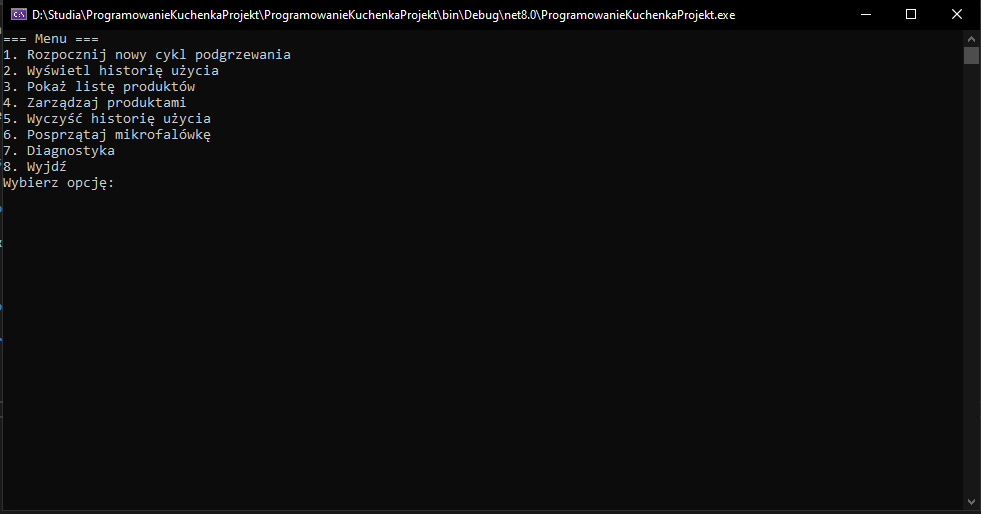
\includegraphics[width=0.9\textwidth]{EkranPowitalny.png}
      \caption{Lista możliwych interakcji}
    \label{fig:example}
\end{figure}

Po uruchomieniu programu pojawia nam się menu z listą możliwych wyborów.

\newpage

\section{Rozpoczęcie podgrzewania}

\begin{figure}[h]
    \centering
    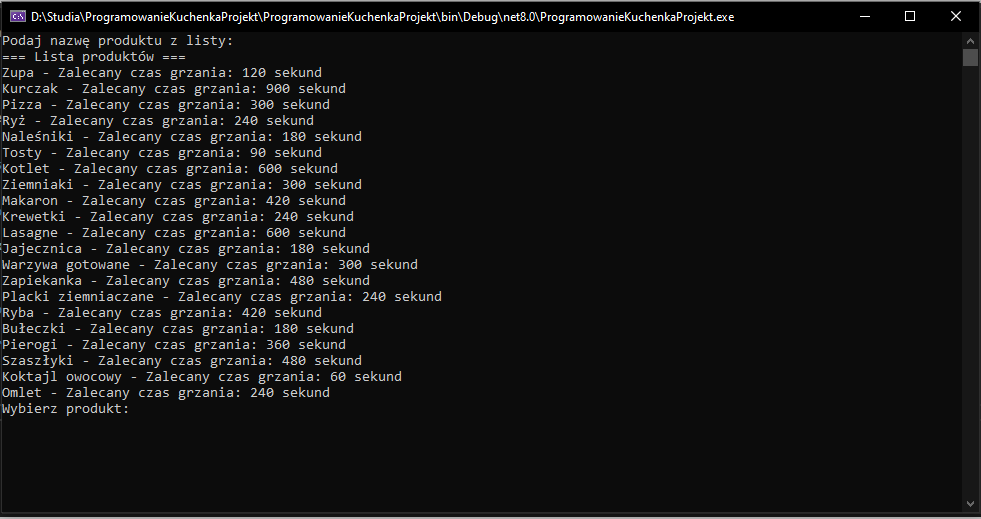
\includegraphics[width=0.9\textwidth]{Menu1.png}
      \caption{Wyświetla listę produktów które można podgrzać}
    \label{fig:example}
\end{figure}

Po wejściu w menu produktów do podgrzania trzeba podać czas podgrzewania oraz potwierdzić rozpoczęcie. 

\subsection{Zakończenie podgrzewania}
\begin{figure}[h]
    \centering
    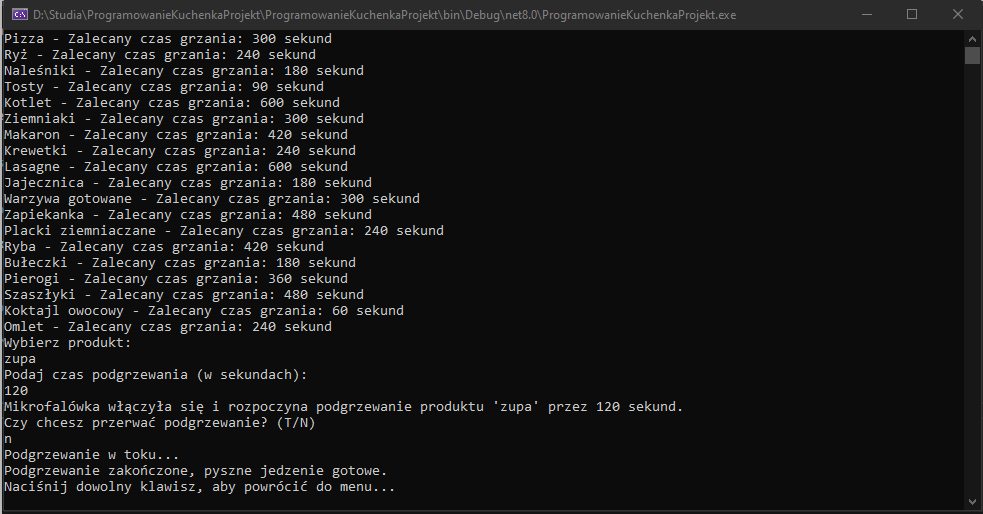
\includegraphics[width=0.9\textwidth]{Menu2.png}
      \caption{Menu po zakończeniu podgrzewania}
    \label{fig:example}
\end{figure}

Po zakończeniu podgrzewania program zwraca nam informację, czy jedzenie jest dobrze przygotowane, czy coś poszło nie tak.

\newpage

\subsection{Historia podgrzewania}
\begin{figure}[h]
    \centering
    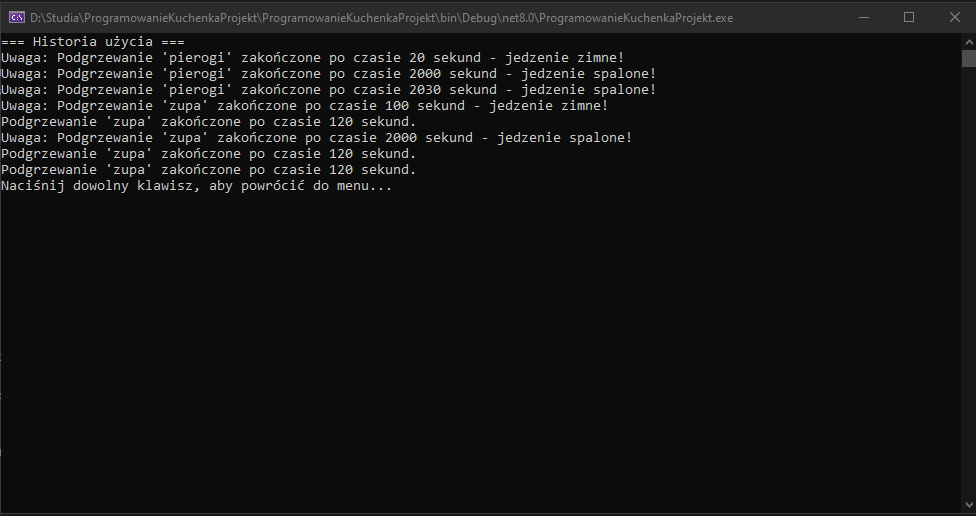
\includegraphics[width=0.9\textwidth]{Menu3.png}
      \caption{Historia}
    \label{fig:example}
\end{figure}

Po wybraniu pozycji numer 2 wyświetla nam się historia podgrzewania z informacjami o produkcie, czasie podgrzewania i jakości jedzenia. 

\subsection{Wyświetlanie listy produktów}
\begin{figure}[h]
    \centering
    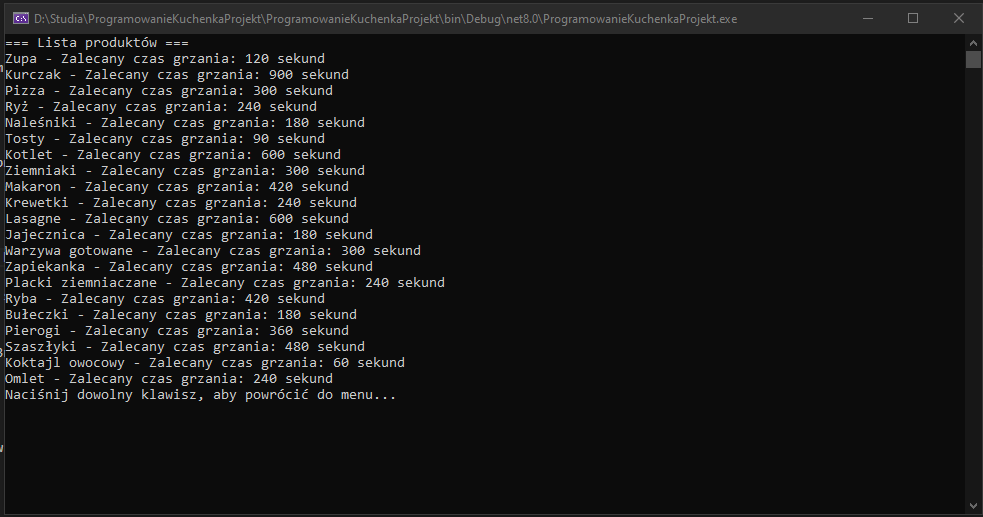
\includegraphics[width=0.9\textwidth]{Menu4.png}
      \caption{Lista produktów}
    \label{fig:example}
\end{figure}

Po wybraniu numeru 3 wyświetli nam się lista dostępnych produktów. 

\newpage

\subsection{Zarządzanie produktami}


\begin{figure}[h]
    \centering
    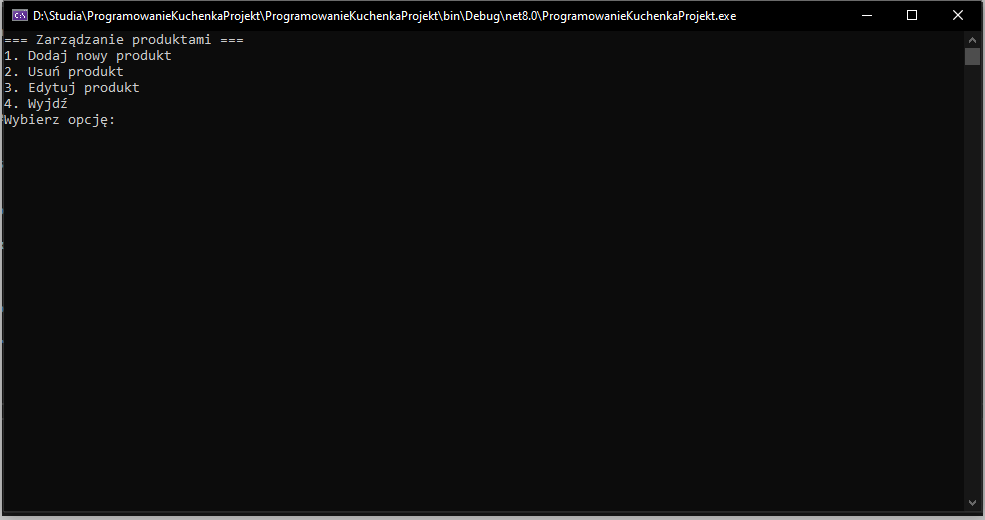
\includegraphics[width=0.9\textwidth]{Menu5.png}
      \caption{Menu zarządzania}
    \label{fig:example}
\end{figure}

Po wybraniu numeru 4 mamy dostęp do zarządzania listą produktów, możemy dodać, usunąć lub edytować pozycje.

\subsection{Dodanie produktu}
\begin{figure}[h]
    \centering
    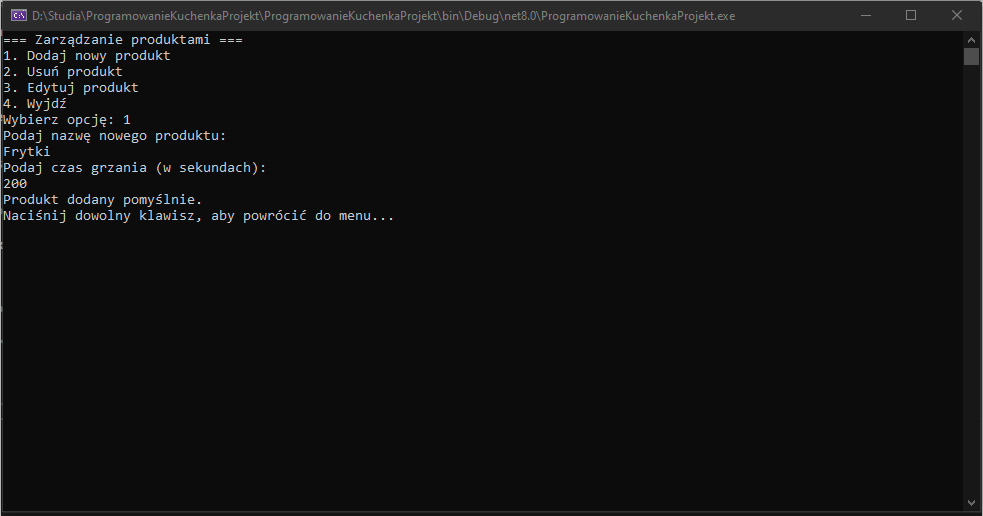
\includegraphics[width=0.9\textwidth]{Menu6.png}
      \caption{Dodanie produktu do systemu}
    \label{fig:example}
\end{figure}

Produkt został pomyślnie dodany do bazy.

\newpage
\subsubsection{Błąd przy dodawaniu produktu}
\begin{figure}[h]
    \centering
    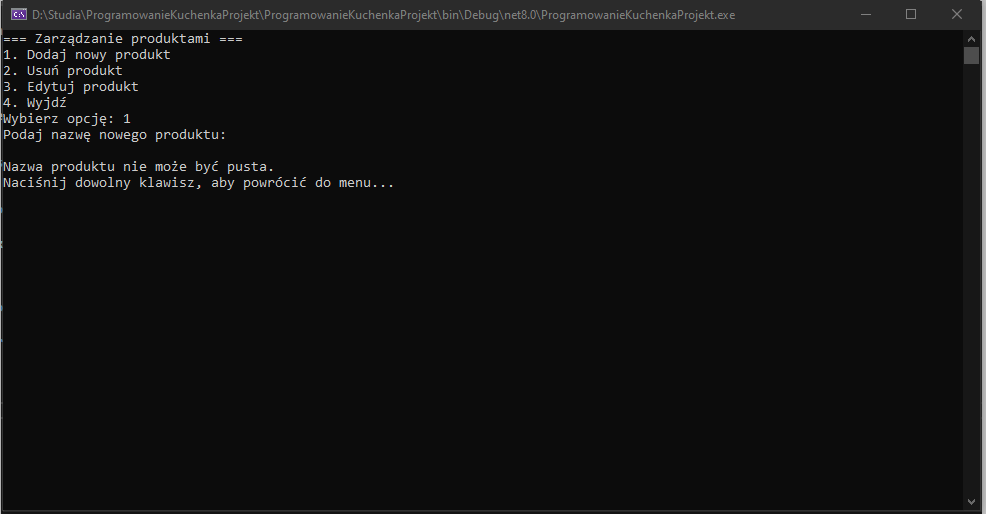
\includegraphics[width=0.9\textwidth]{Menu7.png}
      \caption{Błąd dodania, nazwa pusta}
    \label{fig:example}
\end{figure}

Przy dodawaniu produktu nazwa nie może być pusta.

\subsubsection{Błąd przy dodawaniu produktu}
\begin{figure}[h]
    \centering
    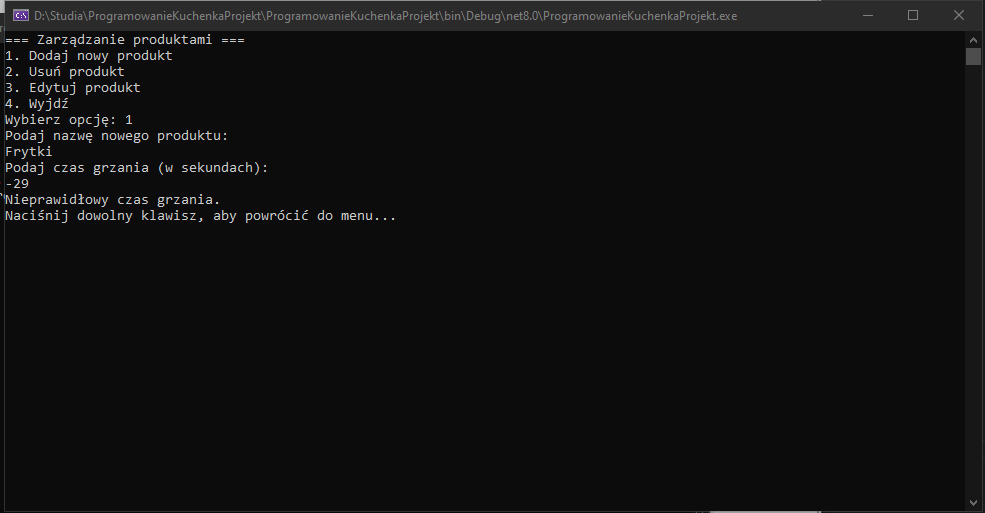
\includegraphics[width=0.9\textwidth]{Menu8.png}
      \caption{Błąd dodania, czas ujemny}
    \label{fig:example}
\end{figure}

Przy dodawaniu produktu czas podgrzewania nie może być równy 0 lub ujemny.

\newpage

\subsection{Aktualizowanie produktu}

\begin{figure}[h]
    \centering
    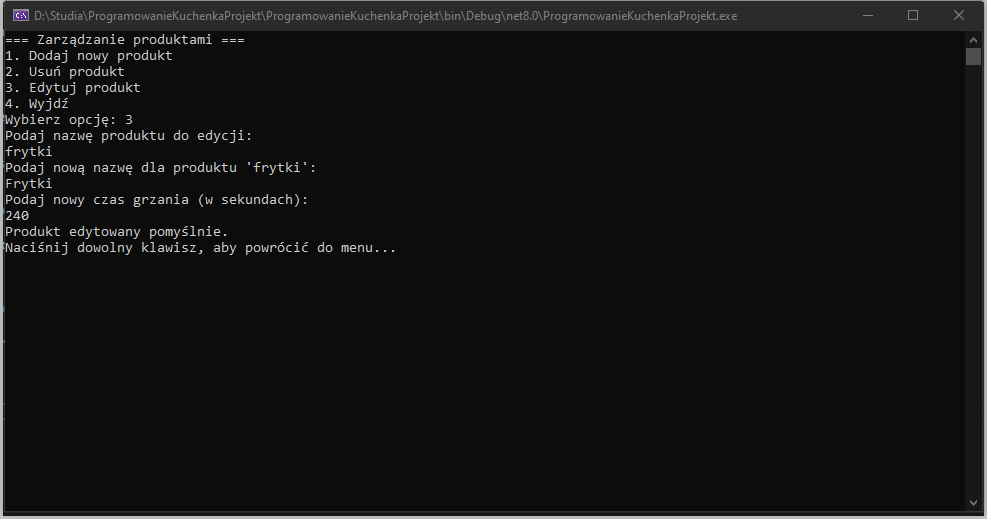
\includegraphics[width=0.9\textwidth]{Menu9.png}
      \caption{Aktualizacja produktu pomyślna}
    \label{fig:example}
\end{figure}

Aktualizując produkt możemy zmienić jego nazwę lub czas podgrzewania.

\subsubsection{Błędna aktualizacja produktu}

\begin{figure}[h]
    \centering
    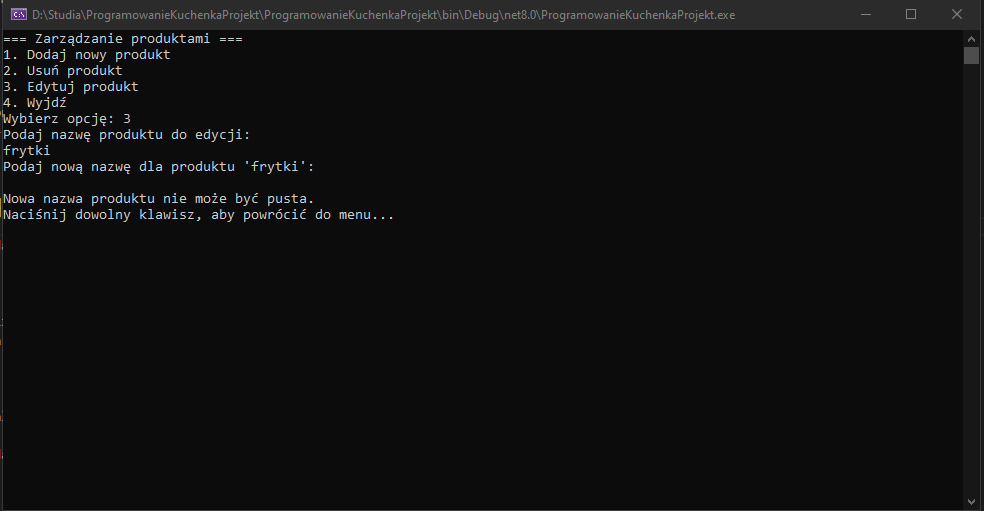
\includegraphics[width=0.9\textwidth]{Menu10.png}
      \caption{Błąd, pusta nazwa}
    \label{fig:example}
\end{figure}

Przy aktualizacji, tak samo jak przy dodawaniu program sprawdza czy nazwa jest pusta oraz czas podgrzewania dodatni.
\newpage
\subsection{Czyszczenie historii podgrzewania}

\begin{figure}[h]
    \centering
    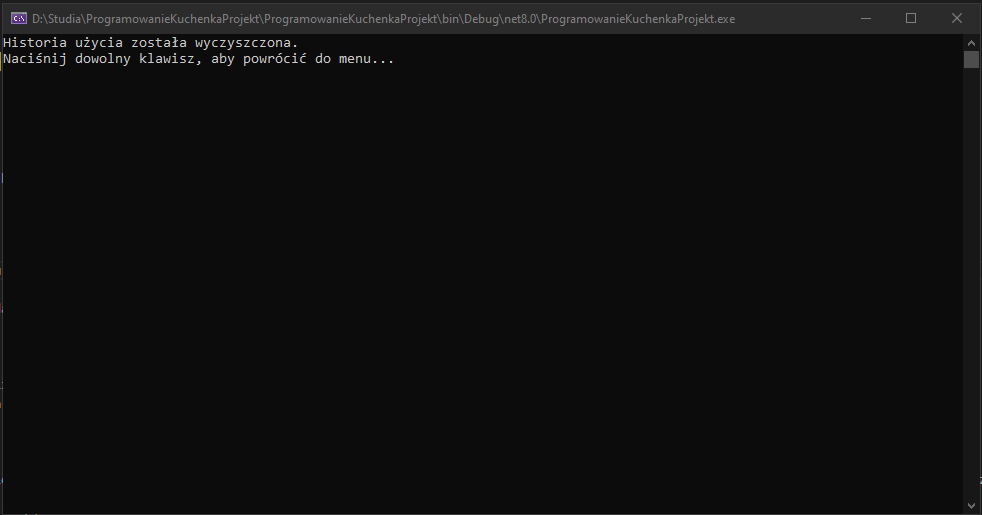
\includegraphics[width=0.9\textwidth]{Menu11.png}
      \caption{Historia została wyczyszczona}
    \label{fig:example}
\end{figure}

Program pozwala na wyczyszczenie historii podgrzewania.

\subsection{Wymóg czyszczenia mikrofalówki}

\begin{figure}[h]
    \centering
    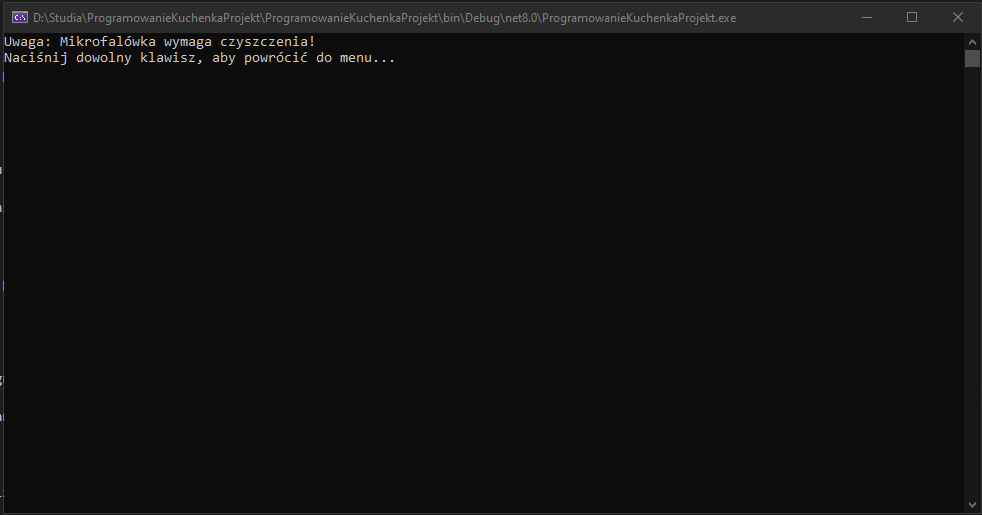
\includegraphics[width=0.9\textwidth]{Menu12.png}
      \caption{Mikrofalówka wymaga czyczszczenia}
    \label{fig:example}
\end{figure}

Po 5 użyciach mikrofalówka wymaga czyszczenia, aby nadal móc jej używać.
\newpage
\subsubsection{Czyszczenie mikrofalówki}

\begin{figure}[h]
    \centering
    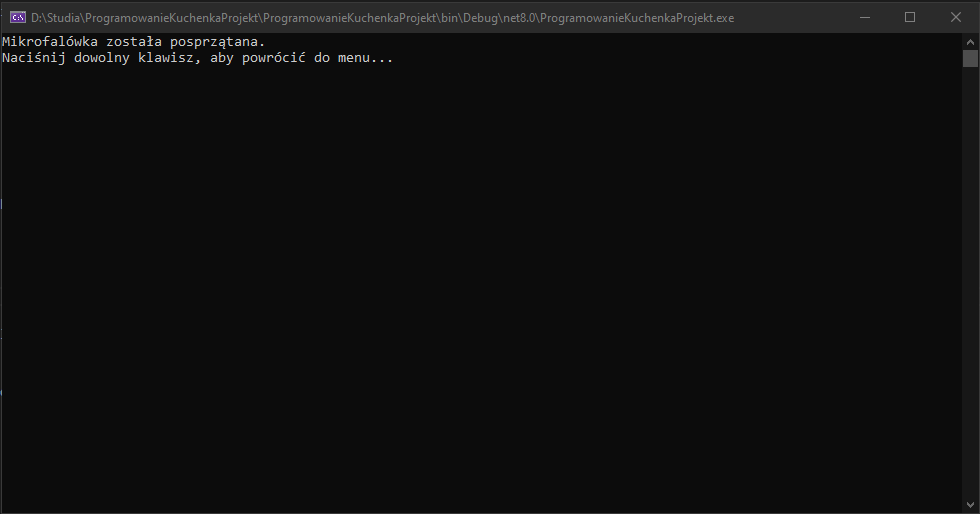
\includegraphics[width=0.9\textwidth]{Menu13.png}
      \caption{Mikrofalówka wyczyszczona}
    \label{fig:example}
\end{figure}

Po wybraniu opcji numer 6 mikrofalówka zostaje wyczyszczona i można znów ją używać.

\subsection{Diagnostyka}
\begin{figure}[h]
    \centering
    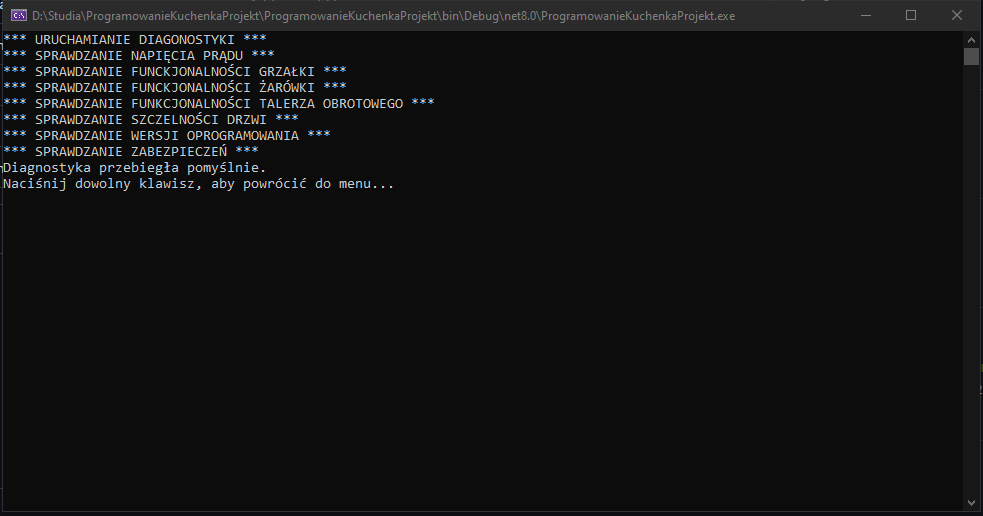
\includegraphics[width=0.9\textwidth]{Menu14.png}
      \caption{Diagnostyka pomyślna}
    \label{fig:example}
\end{figure}

Po wybraniu opcji numer 7 mikrofalówka przeprowadza diagnostykę, może ona zakończyć się pomyślnie lub znaleźć błąd.
\newpage
\subsubsection{Diagnostyka wykryła błąd}

\begin{figure}[h]
    \centering
    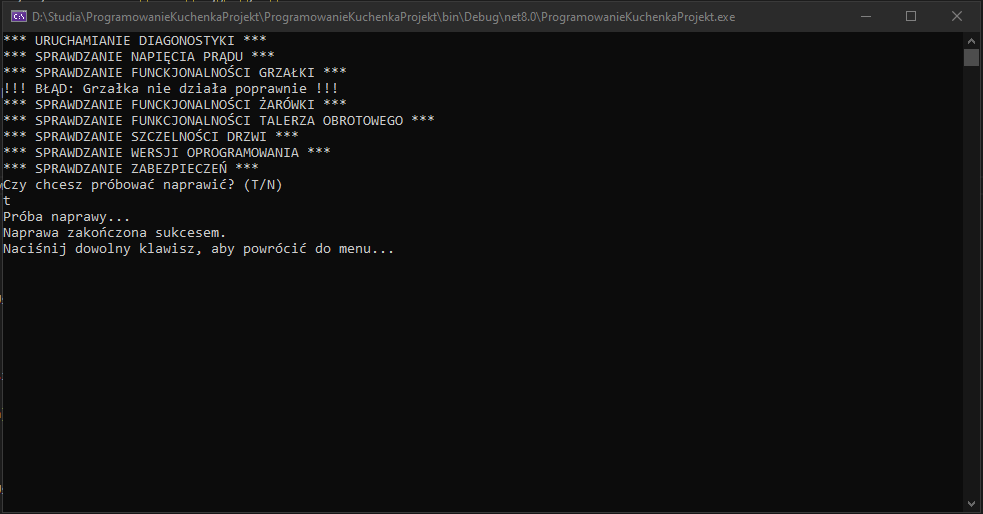
\includegraphics[width=0.9\textwidth]{Menu15.png}
      \caption{Błąd grzałki}
    \label{fig:example}
\end{figure}
Po wykryciu błędu można spróbować go naprawić, po czym zostaje podjęta próba naprawy.